\documentclass{article}
% For math environments
\usepackage{amsmath, amsfonts}
% For links
\usepackage[hidelinks]{hyperref}
% So space it put between paragraphs
\usepackage{parskip}
% For figures
\usepackage{tikz}
% Set the margins to not be ridiculous
\usepackage[margin=0.75in]{geometry}
% For multiple columns
\usepackage{multicol}
% For controlling enum/itemize spacing and indentation
\usepackage{enumitem}

% For tikz plots
\usepackage{pgfplots}
% This isn't needed but avoids a compiler warning
\pgfplotsset{compat=1.16}

% Allow multi-line equations to be broken across pages
\allowdisplaybreaks

% Use @ as a letter
\makeatletter

% Scale down all tikz coordinates while maintaining font size
\tikzset{every picture/.style={scale=0.45, every picture/.style={}}}


% Macros
% Monospace code
\def\code#1{\texttt{#1}}

% Greek letters
\def\a{\alpha}
\def\b{\beta}
\def\g{\gamma}
\def\d{\delta}
\def\D{\Delta}

% Some common sets
\def\es{\varnothing}
\def\ints{{\mathbb{Z}}}

% Commands that make life easier
\newcommand\gath[1]{\begin{gather} #1 \end{gather}}
\newcommand\gaths[1]{\begin{gather*} #1 \end{gather*}}
\newcommand\ali[1]{\begin{align} #1 \end{align}}
\newcommand\parens[1]{\left( #1 \right)}
\newcommand\squares[1]{\left[ #1 \right]}
\newcommand\braces[1]{\left\{ #1 \right\}}
\newcommand\angles[1]{\left\langle #1 \right\rangle}
\newcommand\deriv[2]{\frac{d #1}{d #2}}
\newcommand\abs[1]{\left| #1 \right|}
\newcommand\floor[1]{\left\lfloor #1 \right\rfloor}
\newcommand\ceil[1]{\left\lceil #1 \right\rceil}
\DeclareMathOperator{\lcm}{lcm}
\def\non{\nonumber \\}
\newcommand\unit[1]{~\mathrm{#1}}
\newcommand\combos[2]{{}_{#1}C_{#2}}

% Set stuff
\def\ss{\subseteq}

% Multiline equation space
\def\mlesp{\hspace{1.2cm}}

% For grid diagrams
\newcommand\gridbox[3]{\draw (#1,#2) rectangle (#1+1,#2+1) node[pos=.5] {#3};}
\newcommand\gridboxh[3]{\draw[fill=red!20] (#1,#2) rectangle (#1+1,#2+1) node[pos=.5] {#3};}
\newcommand\gridboxb[3]{\draw[fill=black] (#1,#2) rectangle (#1+1,#2+1) node[pos=.5] {#3};}
\newcommand\gridsym[3]{\node at (#1+0.5,#2+0.5) {$#3$};}
\newcommand\gridblank[2]{\filldraw[draw=gray, color=gray] (#1,#2) rectangle (#1+1,#2+1);}
\newcommand\gridcirc[2]{\draw (#1 + 0.5,#2 + 0.5) circle (0.25);}
\newcommand\cwlab[3]{
  \def\dd{0.15}
  \draw (#1 + \dd - 0.03, #2 + 1 - \dd) node {\scriptsize #3};
}

\def\bbw{3.5}
\def\bbh{2}
\newcommand\bigbox[3]{\draw (#1*\bbw,#2*\bbh) rectangle (#1*\bbw+\bbw,#2*\bbh+\bbh) node[pos=.5] {#3};}
\newcommand\bbtextr[3]{\node[right] at (#1*\bbw,#2*\bbh+0.5*\bbh) {#3};}
\newcommand\bbtextb[3]{\node[align=center] at (#1*\bbw+0.5*\bbw,#2*\bbh+0.5*\bbh) {#3};}

% Box puzzle stock answer
\newcommand\boxans[1]{
  Logic was used to deduce the solution:

  #1

  This was verified using Python as well as shown to be unique with a brute force approach.
}

% Standard crossnumber grid
\newcommand\crossnumstd[9]{
  \begin{center}
    \begin{tikzpicture}[scale=2]
      \gridbox{0}{2}{#1}
      \gridbox{1}{2}{#2}
      \gridbox{2}{2}{#3}
      \gridbox{0}{1}{#4}
      \gridbox{1}{1}{#5}
      \gridbox{2}{1}{#6}
      \gridbox{0}{0}{#7}
      \gridbox{1}{0}{#8}
      \gridbox{2}{0}{#9}

      % Labels
      \cwlab{0}{2}{1}
      \cwlab{1}{2}{2}
      \cwlab{2}{2}{3}
      \cwlab{0}{1}{4}
      \cwlab{0}{0}{5}
    \end{tikzpicture}
  \end{center}
}

% Multiple numbers
\newcommand\mn[1]{$#1$'s}

% Commands for problems
\newcommand\problem[4]{
\section*{#1}

\textbf{Question:} #3

\textbf{Answer:} #2

\textbf{Explanation:} #4
}
\newcommand\aproblem[4]{\problem{Dec #1}{#2}{#3}{#4}}
\newcommand\cproblem[4]{\problem{Problem #1}{#2}{#3}{#4}}

\newcommand\xref@advent[2]{#1 Advent, Dec~#2 problem}
\newcommand\xref@card[2]{#1 Christmas Card, Problem #2}

% For answered verified with Python
\newcommand{\verified}{This was verified with a brute-force Python program.}

\def\advent@xxi@i{
  The geometric mean of a set of $n$ numbers can be computed by multiplying together all the numbers then computing the $n$th root of the result.

  The factors of $4$ are $1$, $2$ and $4$. The geometric mean of these is 2.

  The factors of $6$ are $1$, $2$, $3$, and $6$. The geometric mean of these is $\sqrt{6}$.

  The geometric mean of all the factors of today's number is $22$.
}

\def\advent@xxi@ii{
  The number $7n$ has $37$ factors (including $1$ and the number itself).
  How many factors does $8n$ have?
}

\def\advent@xxi@iii{
  If you write out the numbers from $1$ to $1000$ (inclusive), how many times will you write the digit $0$?
}

\def\advent@xxi@iv{
  Put the digits $1$ to $9$ (using each digit exactly once) in the boxes so that the sums are correct.
  The sums should be read left to right and top to bottom ignoring the usual order of operations.
  For example, $4 + 3 \times 2$ is $14$, not $10$.
  Today's number is the product of the numbers in the red boxes.

  \grid@advent@xxi@iv{}{}{}{}{}{}{}{}{}
}

\def\advent@xxi@v{
  How many different isosceles triangles are there whose perimeter is $50$ units, and whose area is an integer number of units squared?

  (Two triangles that are rotations, reflections and translations of each other are counted as the same triangle. Triangles with an area of 0 should not be counted.)
}

\def\advent@xxi@vi{
  When $12345$ is divided by today's number, the remainder is $205$.
  When $6789$ is divided by today's number, the remainder is $112$.
}

\newcommand\dec@ai{0.30901699437494745}
\newcommand\dec@aii{0.8090169943749475}
\newcommand\dec@bi{0.5877852522924731}
\newcommand\dec@bii{0.9510565162951535}
\newcommand\decagon[5]{
  \def\ai{\dec@ai*#3+#1}
  \def\aii{\dec@aii*#3+#1}
  \def\bi{\dec@bi*#3+#2}
  \def\bii{\dec@bii*#3+#2}
  \draw (#3+#1, #2) -- (\aii, \bi) -- (\ai, \bii) -- (-\ai, \bii) -- (-\aii, \bi) -- (-#3+#1, #2) -- (-\aii, -\bi) -- (-\ai, -\bii) -- (\ai, -\bii) -- (\aii, -\bi) -- cycle;
  \fill[fill=red] (-\ai, -\bii) -- (#4*#3+#1, #5*#3+#2) -- (\ai, -\bii) -- cycle;
}
\def\advent@xxi@vii{
  The picture below shows eight regular decagons.
  In each decagon, a red triangle has been drawn with vertices at three of the vertices of the decagon.

  \begin{center}
    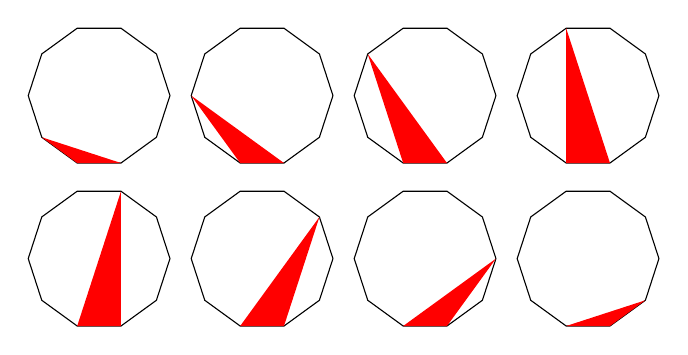
\begin{tikzpicture}
      \def\dr{2}
      \def\spc{2.3*\dr}

      \decagon{0*\spc}{\spc}{\dr}{-\dec@aii}{-\dec@bi}
      \decagon{1*\spc}{\spc}{\dr}{-1}{0}
      \decagon{2*\spc}{\spc}{\dr}{-\dec@aii}{\dec@bi}
      \decagon{3*\spc}{\spc}{\dr}{-\dec@ai}{\dec@bii}

      \decagon{0*\spc}{0}{\dr}{\dec@ai}{\dec@bii}
      \decagon{1*\spc}{0}{\dr}{\dec@aii}{\dec@bi}
      \decagon{2*\spc}{0}{\dr}{1}{0}
      \decagon{3*\spc}{0}{\dr}{\dec@aii}{-\dec@bi}
    \end{tikzpicture}
  \end{center}

  The area of each decagon is $240$.
  What is the total area of all the red triangles?
}

\def\advent@xxi@viii{
  The sum of three integers is $51$.
  The product of the same three integers is $836$. What is the product of largest integer and the second-largest integer?
}

\def\advent@xxi@ix{
  Eve writes down a sequence of consecutive positive integers (she writes more than one number).
  The sum of the numbers Eve has written down is $844$.
  Today's number is the smallest integer that Eve has written down.
}

\def\advent@xxi@x{
  Put the digits $1$ to $9$ (using each digit exactly once) in the boxes so that the sums are correct.
  Today's number is the largest number you can make using the digits in the red boxes.

  \grid@advent@xxi@x{}{}{}{}{}{}{}{}{}
}

\def\advent@xxi@xi{
  The integers are written in a triangle as shown below:
  \begin{center}
    \begin{tabular}{ccccccc}
         &    &    & 1    &    &    &    \\
         &    & 2  & 3    & 4  &    &    \\
         & 5  & 6  & 7    & 8  & 9  &    \\
      10 & 11 & 12 & 13   & 14 & 15 & 16 \\
         &    &    & etc. &    &    &
    \end{tabular}
  \end{center}
  Today's number appears directly above the number $750$ in the triangle of integers.
}

\def\advent@xxi@abgrid{
  \begin{center}
    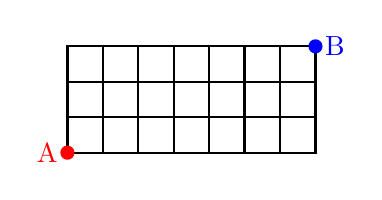
\begin{tikzpicture}
      \def\gs{1}
      % Grid
      \foreach \i in {0,...,6}{
          \foreach \j in {0,...,2}{
              \draw[thick] (\i * \gs, \j * \gs) rectangle (\i * \gs + \gs, \j * \gs + \gs);
            }
        }
      % Points
      \fill[color=red] (0, 0) circle (0.2) node[color=red,left] {A};
      \fill[color=blue] (7*\gs, 3*\gs) circle (0.2) node[color=blue,right] {B};
    \end{tikzpicture}
  \end{center}
}
\def\advent@xxi@xii{
  You start at the point marked A in the picture below. You want to get to the point marked B.
  You may travel \textbf{to the right} or \textbf{upwards} along the black lines.

  \advent@xxi@abgrid

  Today's number is the total number of possible routes to get from A to B.
}

\def\advent@xxi@xiii{
  The diagram below shows three circles and two triangles.
  The three circles all meet at one point.
  The vertices of the smaller red triangle are at the centers of the circles.
  The lines connecting the vertices of the larger blue triangle to the point where all three circles meet are diameters of the three circles.

  \begin{center}
    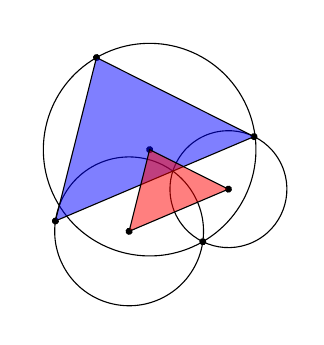
\begin{tikzpicture}[rotate=30,transform shape]
      \def\bcr{3}
      \def\scr{0.55*\bcr}
      \def\sca{34}
      \def\mcr{0.7*\bcr}
      \def\mca{142}
      \def\pr{0.1}

      % Circles
      \draw (0, \bcr) circle (\bcr);
      \draw (\sca: \scr) circle (\scr);
      \draw (\mca: \mcr) circle (\mcr);

      % Points
      \fill (0, 0) circle (\pr);
      \fill (0, \bcr) circle (\pr);
      \fill (0, 2*\bcr) circle (\pr);
      \fill (\sca: \scr) circle (\pr);
      \fill (\sca: 2*\scr) circle (\pr);
      \fill (\mca: \mcr) circle (\pr);
      \fill (\mca: 2*\mcr) circle (\pr);

      % Triangles
      \draw[fill=blue,fill opacity=0.5] (\mca: 2*\mcr) -- (0, 2*\bcr) -- (\sca: 2*\scr) -- cycle;
      \draw[fill=red,fill opacity=0.5] (\mca: \mcr) -- (0, \bcr) -- (\sca: \scr) -- cycle;
    \end{tikzpicture}
  \end{center}

  The area of the smaller red triangle is $226$.
  What is the area of the larger blue triangle?
}

\def\advent@xxi@xiv{
  You start at the point marked A in the picture below.
  You want to get to the point marked B.
  You may travel \textbf{to the right}, \textbf{upwards}, or \textbf{to the left} along the black lines, but you cannot pass along the same line segment more than once.

  \advent@xxi@abgrid

  Today's number is the total number of possible routes to get from A to B.
}

\newcommand\pyramid@advent@xxi@xvi[6]{
  \begin{center}
    \begin{tabular}{cccccc}
      (row 1) &    &    & #1   &    &    \\
      (row 2) &    & #2 &      & #3 &    \\
      (row 3) & #4 &    & #5   &    & #6 \\
              &    &    & etc. &    &
    \end{tabular}
  \end{center}
}
\def\advent@xxi@xv{
  The odd numbers are written in a pyramid.

  \pyramid@advent@xxi@xvi{1}{3}{5}{7}{9}{11}

  What is the mean of the numbers in the 19th row?
}

\newcommand\grid@advent@xxi@xvi[9]{
  \begin{center}
    \begin{tikzpicture}[scale=2]
      \gridbox{0}{2}{#1}
      \gridbox{1}{2}{#2}
      \gridbox{2}{2}{#3}
      \gridbox{0}{1}{#4}
      \gridbox{1}{1}{#5}
      \gridbox{2}{1}{#6}
      \gridbox{0}{0}{#7}
      \gridbox{1}{0}{#8}
      \gridbox{2}{0}{#9}

      % Labels
      \cwlab{0}{2}{1}
      \cwlab{1}{2}{2}
      \cwlab{2}{2}{3}
      \cwlab{0}{1}{4}
      \cwlab{0}{0}{5}
    \end{tikzpicture}
  \end{center}
}
\def\advent@xxi@xvi{
  Each clue in this crossnumber is formed of two parts connected by a logical connective: AND means that both parts are true; NAND means that at most one part is true; OR means that at least one part is true; NOR means that neither part is true; XOR means that exactly one part is true; XNOR means that either both parts are false or both parts are true.
  No number starts with $0$.

  \begin{multicols}{2}
    \grid@advent@xxi@xvi{}{}{}{}{}{}{}{}{}

    \columnbreak

    \begin{enumerate}
      \item \textbf{1A} is a palindrome XNOR \textbf{1D} is a palindrome.
      \item \textbf{1A} is greater than $350$ NOR \textbf{1D} is less than $150$.
      \item \textbf{3D} is odd NAND \textbf{4A} and \textbf{2D} are equal.
      \item \textbf{3D} is prime XOR \textbf{5A} is odd.
      \item \textbf{4A} is a cube AND \textbf{2D} is a cube.
      \item The sum of the digits of \textbf{3D} is $2$ OR the sum of the digits of \textbf{5A} is $5$.
      \item Today's number is \textbf{1D}.
    \end{enumerate}
  \end{multicols}
}

\def\advent@xxi@xvii{
  The digital product of a number is computed by multiplying together all of its digits. For example, the digital product of $6273$ is $252$.

  Today's number is the smallest number whose digital product is $252$.
}

\def\advent@xxi@xviii{
  Put the digits $1$ to $9$ (using each digit exactly once) in the boxes so that the sums are correct.
  The sums should be read left to right and top to bottom ignoring the usual order of operations.
  For example, $4 + 3 \times 2$ is $14$, not $10$.
  Today's number is the product of the numbers in the red boxes.

  \grid@advent@xxi@xviii{}{}{}{}{}{}{}{}{}
}

\def\advent@xxi@xix{
  The equation $352x^3 - 528x^2 + 90 = 0$ has three distinct real-valued solutions.

  Today's number is the number of integers $a$ such that the equation $352x^3 - 528x^2 + a = 0$ has three distinct real-valued solutions.
}

\def\advent@xxi@xx{
  What is the area of the largest area triangle that has one side of length $32$ and one side of length $19$?
}

\newcommand\grid@advent@xxi@xxi[9]{
  \begin{center}
    \begin{tikzpicture}
      \bigbox{0}{3}{#1}
      \bigbox{1}{3}{#2}
      \bigbox{2}{3}{#3}
      \bbtextr{3}{3}{\textbf{today's number}}

      \bigbox{0}{2}{#4}
      \bigbox{1}{2}{#5}
      \bigbox{2}{2}{#6}
      \bbtextr{3}{2}{prime}

      \bigbox{0}{1}{#7}
      \bigbox{1}{1}{#8}
      \bigbox{2}{1}{#9}
      \bbtextr{3}{1}{square}

      \bbtextb{0}{0}{cube}
      \bbtextb{1}{0}{odd}
      \bbtextb{2}{0}{multiple\\of $11$}
    \end{tikzpicture}
  \end{center}
}
\def\advent@xxi@xxi{
  Arrange the digits $1$–$9$ (using each digit exactly once) so that the three digit number in: the middle row is a prime number; the bottom row is a square number; the left column is a cube number; the middle column is an odd number; the right column is a multiple of $11$.
  The $3$-digit number in the first row is today's number.

  \grid@advent@xxi@xxi{}{}{}{}{}{}{}{}{}
}

\def\advent@xxi@xxii{
  There are $12$ ways of placing $2$ tokens on a $2 \times 4$ grid so that no two tokens are next to each other horizontally, vertically or diagonally:

  \begin{center}
    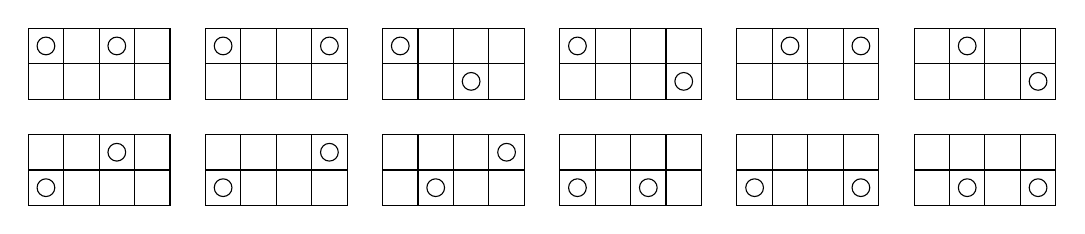
\begin{tikzpicture}
      % Draw all the grids
      \foreach \gi in {0,1}{
          \foreach \gj in {0,...,5}{
              \foreach \i in {0,1}{
                  \foreach \j in {0,...,3}{
                      \gridbox{5*\gj + \j}{3*\gi + \i}{}
                    }
                }
            }
        }

      % Place token circles
      \gridcirc{0}{4}
      \gridcirc{2}{4}
      \gridcirc{5}{4}
      \gridcirc{8}{4}
      \gridcirc{10}{4}
      \gridcirc{12}{3}
      \gridcirc{15}{4}
      \gridcirc{18}{3}
      \gridcirc{21}{4}
      \gridcirc{23}{4}
      \gridcirc{26}{4}
      \gridcirc{28}{3}
      \gridcirc{0}{0}
      \gridcirc{2}{1}
      \gridcirc{5}{0}
      \gridcirc{8}{1}
      \gridcirc{11}{0}
      \gridcirc{13}{1}
      \gridcirc{15}{0}
      \gridcirc{17}{0}
      \gridcirc{20}{0}
      \gridcirc{23}{0}
      \gridcirc{26}{0}
      \gridcirc{28}{0}
    \end{tikzpicture}
  \end{center}

  Today's number is the number of ways of placing $2$ tokens on a $2 \times 21$ grid so that no two tokens are next to each other horizontally, vertically or diagonally.
}

\def\advent@xxi@xxiii{
  I draw the parabola $y = x^2$ and mark points on the parabola at $x = 17$ and $x = -6$.
  I then draw a straight line connecting these two points.

  At which value of $y$ does this line intercept the $y$-axis?
}

\def\advent@xxi@xxiv{
  The digital product of a number is computed by multiplying together all of its digits.
  For example, the digital product of $1522$ is $20$.

  How many $12$-digit numbers are there whose digital product is $20$?
}

\def\card@xxi@i{
  What is the sum of all the odd integers between $0$ and $30$?
}

\def\card@xxi@ii{
  What is the sum of all the odd integers between $0$ and $5668$?
}

\def\card@xxi@iii{
  What is the smallest integer with a digital sum of $28$ and a digital product of $10000$?
}

\def\card@xxi@iv{
  What is the smallest integer with a digital sum of $41$ and a digital product of $432000$?
}

\def\card@xxi@v{
  What is the area of the largest area dodecagon that will fit inside a circle with area $111185 \pi$?
}

\def\card@xxi@vi{
  What is the area of the largest area heptagon that will fit inside a semicircle with area $115185 \pi$?
}

\def\card@xxi@vii{
  How many terms are there in the (simplified) expansion of $(x + y + z)^2$?
}

\def\card@xxi@viii{
  How many terms are there in the (simplified) expansion of $(x + y + z)^{41172}$?
}

\def\card@xxi@ix{
  What is the largest integer that cannot be written as $4a + 5b$ for non-negative integers $a$ and $b$?
}

\def\card@xxi@x{
  What is the largest integer that cannot be written as $83409a + 66608b$ for non-negative integers $a$ and $b$?
}

\def\card@xxi@xi{
  How many positive integers are there below $100$ whose digits are all non-zero and different?
}

\def\card@xxi@xii{
  How many positive integers are there whose digits are all non-zero and different?
}

\def\card@xxi@xiii{
  What is the only integer for which taking the geometric mean of all its factors (including $1$ and the number itself) gives $2$?
}

\def\card@xxi@xiv{
  What is the only integer for which taking the geometric mean of all its factors (including $1$ and the number itself) gives $25$?
}

\input{boxes}

\begin{document}

\title{MS Scroggs Advent Calendar 2022 Answers}
\author{Dan Whitman}
\date{}

\maketitle

% TODO: Once the event is over, add answers link.
%Answers: \href{https://www.mscroggs.co.uk/puzzles/advent2021}{https://www.mscroggs.co.uk/puzzles/advent2021}
Synchronized calendar: \href{http://mscroggs.co.uk/adventcode/JYcziCbI}{http://mscroggs.co.uk/adventcode/JYcziCbI}

\aproblem{1}{162}{\advent@xxii@i}{
  Since $p_1 = (9,0)$ is a vertex and the $y$-axis is a line of symmetry, it must be that a second vertex is $p_2 = (-9, 0)$.
  Since there must be four vertices, and both $p_1$ and $p_2$ are on the $x$-axis, it must be that the other two vertices are on the $y$-axis.
  This is because any vertex not on either axis would result in four vertices not on either axis due to the axes being lines of symmetry, and a rectangle cannot have six vertices!
  It then must be that the two $y$-axis vertices are at $p_3 = (0, 9)$ and $p_4 = (0, -9)$, since any other points that possess the required symmetry would result in a parallelogram without right angles.

  Therefore, our rectangle is also square that clearly has sides of $s = \sqrt{9^2 + 9^2} = 9\sqrt{2}$.
  The area is then of course $A = s^2 = 81 \cdot 2 = 162$.
}

\aproblem{2}{840}{\advent@xxii@ii}{
  Clearly $1$, $2$, $3$, $5$, and $7$ are prime whereas $4 = 2^2$, $6 = 2 \cdot 3$, and $8 = 2^3$.
  Therefore we have that
  \gath{
    \lcm(1, 2, 3, 4, 5, 6, 7, 8) = 2^3 \cdot 3 \cdot 5 \cdot 7 = 840 \,.
  }
}

\aproblem{3}{369}{\advent@xxii@iii}{
  Suppose that for the $n$th row we choose the element in the $p_n$th column (where $1 \leq n, p_n \leq 9$).
  Since we must only choose exactly one number in each column, clearly for any permutation we have that $\braces{p_n \mid 1 \leq n \leq 9} = \braces{1, 2, \ldots, 9}$, and hence
  \gath{
    \sum_{n=1}^9 p_n = 1 + 2 + \ldots + 9 = \sum_{i=1}^9 i = \frac{9 \cdot 10}{2} = 45 \,.
  }
  Now, if $x_n$ is the selected value of the $n$th row, then this value is reasoned to be
  \gath{
    x_n = 9(n-1) + p_n \,.
  }
  Hence, the sum of all the selected values is always
  \gath{
    \sum_{n=1}^9 x_n = \sum_{n=1}^9 \squares{9(n-1) + p_n} = 9 \sum_{n=1}^9 n - 9 \sum_{n=1}^9 1 + \sum_{n=1}^9 p_n
    = 9 \cdot 45 - 9 \cdot 9 + 45 = 369
  }
  regardless of the selection permutation.
  This result was verified by a brute force Python program.
}

\aproblem{4}{625}{\advent@xxii@iv}{
  First, clearly the last three digits of any number $n \geq 100$ is just $n \mod 1000$.
  We claim, for all $n \geq 3$, that
  \gath{
    5^n \mod 1000 = \begin{cases}
      625 & \text{$n$ is even}    \\
      125 & \text{$n$ is odd} \,,
    \end{cases}
  }
  which we show by induction on $n$.
  First, for $n = 3$, we obviously have $5^3 = 125 \equiv 125 \pmod{1000}$ so that the hypothesis is true here since $n = 3$ is odd.
  Now suppose that the hypothesis is true for $n$.
  If $n$ is even then $5^n \equiv 625 \pmod{1000}$ so that
  \gath{
    5^{n+1} = 5 \cdot 5^n \equiv 5 \cdot 625 \pmod{1000} \equiv 3125 \pmod{1000} \equiv 125 \pmod{1000},
  }
  which proves the hypothesis for $n+1$ since $n+1$ is odd.
  If, on the other hand, $n$ is odd, then $5^n \equiv 125 \pmod{1000}$ by the induction hypothesis so that
  \gath{
    5^{n+1} = 5 \cdot 5^n \equiv 5 \cdot 125 \pmod{1000} \equiv 625 \pmod{1000},
  }
  which again proves the hypothesis for $n+1$ since here $n+1$ is even.

  Now, since clearly $n = 2022000000$ is even, it follows that the last three digits of $5^n$ are $625$ by what was just proven.
}

\aproblem{5}{315}{\advent@xxii@v}{
  \boxans{\gridsol@advent@xxii@v}
}

\aproblem{6}{128}{\advent@xxii@vi}{
  First, consider a general sum digit $1 \leq s \leq 9$, and let $N_m(s)$ denote the number of $m$-digit numbers such that the digits are all non-zero digits and add to $s$.
  Clearly $N_1(s) = 1$, namely the single digit $s$ itself.
  Next, consider $m$-digit numbers for $m > 1$.
  If the first digit is $1$, then there are $N_{m-1}(s-1)$ combinations of remaining digits so that to overall digital sum is $s$.
  Likewise, if the first digit is $2$, then there are $N_{m-1}(s-2)$ combinations of remaining digits.

  More generally, if the first digit is $1 \leq i \leq s - (m-1)$, then there are $N_{m-1}(s - i)$ combinations of remaining digits such that the overall digital sum is $s$.
  Note that $i \leq s - (m-1)$ since the minimal sum of the remaining digits is $m-1$, namely when they are all \mn{1}.
  Therefore, considering all the first digits, we have the recursive equation
  \gath{
    N_m(s) = \sum_{i=1}^{s - (m-1)} N_{m-1}(s - i) = \sum_{j=m-1}^{s-1} N_{m-1}(j), \label{eqn:06:rec}
  }
  where we have changed indices using $j = s - i$.
  Also note that it must be that $m \leq s$ since there are no terms otherwise, and $m = s$ corresponds to an $s$-digit number with a digital sum $s$ so that all digits must be \mn{1}, and hence $N_s(s) = 1$.

  For a given $s$, it follows that the total number of qualifying integers (with any number of digits) with that digital sum is then
  \gath{
    N_s = \sum_{m=1}^s N_m(s). \label{eqn:06:main}
  }
  Now, we have
  \gath{
    N_2(s) = \sum_{j=1}^{s-1} N_1(j) = \sum_{j=1}^{s-1} 1 = (s - 1) - 1 + 1 = s - 1
  }
  and
  \ali{
    N_3(s) &= \sum_{j=2}^{s-1} N_2(j) = \sum_{j=2}^{s-1} (s - 1) = \sum_{j=2}^{s-1} s - \sum_{j=2}^{s-1} 1 = \squares{\frac{s(s-1)}{2} - 1} - (s - 2) \non
    &= \frac{s(s-1)}{2} - s + 1 = \frac{s(s-1) - 2s + 2}{2} = \frac{s^2 - 3s + 2}{2} = \frac{(s-1)(s-2)}{2}.
  }
  This could be continued to $N_4(s)$, $N_5(s)$, etc., but this would quickly become very tedious.
  In our case we are looking for $N_8$, for which we would need to determine $N_m(s)$ up through $N_8(s)$.
  Rather than endure this tedium, we simply implement the recursive function \eqref{eqn:06:rec} with the base case of $N_1(s) = 1$ in Python and use \eqref{eqn:06:main} to calculate $N_8 = 128$.

  This result was also verified with a brute force search in the Python program.
}

\aproblem{7}{476}{\advent@xxii@vii}{
  It seems fairly clear that the largest triangle that can fit within a hexagon is that whose three vertices lie on every other vertex of the hexagon as shown below:
  \def\hexr{3}
  \begin{center}
    \begin{tikzpicture}
      \draw (-30:\hexr) -- (30:\hexr) -- (90:\hexr) -- (150:\hexr) -- (210:\hexr) -- (270:\hexr) -- cycle;
      \draw[fill=red] (-30:\hexr) -- (90:\hexr) -- (210:\hexr) -- cycle;
    \end{tikzpicture}
  \end{center}
  Let $s$ denote the side length of the hexagon, and let $t$ denote the side of the inner red triangle, which is clearly equilateral.
  The three smaller white triangles inside the hexagon but outside the red triangle are isosceles and have two side of length $s$ and a base of length $t$.
  Moreover, the apex angles of these triangles is $120^\circ$, from which it follows that
  \gath{
    t = \sqrt{3} s
  }
  so that the area of the large red triangle is
  \gath{
    A_t = \frac{\sqrt{3}}{4} t^2 = \frac{\sqrt{3}}{4} \parens{\sqrt{3} s}^2 = \frac{3\sqrt{3}}{4} s^2.
  }
  Meanwhile, the area of the hexagon is
  \gath{
    A_h = \frac{3\sqrt{3}}{2} s^2.
  }
  Therefore, we have
  \gath{
    A_t = \frac{1}{2} A_h = \frac{1}{2} \cdot 952 = 476.
  }
}

\aproblem{8}{840}{\advent@xxii@viii}{
  Suppose that the five real roots are $a$, $b$, $c$, $d$, and $e$ so that the quintic equation is then of course
  \gath{
    (x - a)(x - b)(x - c)(x - d)(x - e) = 0.
  }
  If we were to expand this, clearly the last term is the only term to be a constant without a factor of $x$.
  This expansion would thus have the form
  \gath{
    f(x) + abcde = 0
  }
  such that $f(x)$ is some quintic in which every term has a factor of $x$.
  Therefore, $-f(x) = abcde$, which is exactly the form of the original given equation.
  Hence, the right side is the product of all the roots, which is the answer we seek!

  While not necessary to get the sought answer, we can also use this and a bit of trial and error to quickly and easily find what the roots actually are.
  Our root product $840$ has 32 factors, not including $840$ itself.
  So the roots can be determined by just plugging all the factors into the original quintic and see which result in the equation holding, being careful to also try the negatives of the factors as well.
  This tedious process was implemented in Python to arrive at the five distinct roots $\braces{-4, -3, 2, 5, 7}$.
  It was then verified using Wolfram Alpha that fully expanding the quintic $(x + 4)(x + 3)(x - 2)(x - 5)(x - 7)$ indeed results in the original quintic expression.
}

\aproblem{9}{532}{\advent@xxii@ix}{
  \boxans{\gridsol@advent@xxii@ix}
}

\aproblem{10}{800}{\advent@xxii@x}{
  \def\xmin{\frac{a}{2}}
  Let $f(x) = x^2 - ax$ and $b = -160,000$.
  Clearly the tangent line $y = b$ is perfectly horizontal so that this touches the parabola $f(x)$ when its slope is zero.
  Thus, we have that this occurs at
  \gath{
    f'(x) = 2x - a = 0 \non
    x = \xmin.
  }
  Now, since the parabola must touch the line at this point, it must be that
  \gath{
    f\parens{\xmin} = \parens{\xmin}^2 - a \parens{\xmin} = b \non
    \frac{a^2}{4} - \frac{a^2}{2} = b \non
    \frac{s^2 - 2a^2}{4} = b \non
    -\frac{a^2}{4} = b \non
    a = \sqrt{-4b} = 800.
  }
  This result was verified by plotting $f(x)$ and the line $y = b$ using Python.
}

\aproblem{11}{987}{\advent@xxii@xi}{
  Let $N_1(m)$ denote the number of qualifying $m$-digit numbers that start with a $1$, and let $N_2(m)$ be the number of qualifying $m$-digit numbers that start with a $2$.
  Similarly, let $N(m)$ denote the total number of qualifying $m$-digit numbers.
  Now, if a $m$-digit number starts with a $1$, then the next digit may either be a $1$ \emph{or} a $2$.
  Thus, it follows that
  \gath{
    N_1(m) = \begin{cases}
      1                   & m = 1  \\
      N_1(m-1) + N_2(m-1) & m > 1.
    \end{cases}
    \label{eqn:11:N1rec}
  }
  On the other hand, if an $m$-digit number starts with a $2$, then the next digit \emph{must} be a $1$ so as not to have two \mn{2} in a row.
  Therefore,
  \gath{
    N_2(m) = \begin{cases}
      1        & m = 1 \\
      N_1(m-1) & m > 1 \\
    \end{cases}
    \label{eqn:11:N2rec}
  }
  and also clearly in general
  \gath{
    N(m) = N_1(m) + N_2(m).
  }
  Combining \eqref{eqn:11:N1rec} and \eqref{eqn:11:N2rec} gives
  \gath{
    N_1(m) = \begin{cases}
      1                                         & m = 1 \\
      N_1(1) + N_2(1) = 2                       & m = 2 \\
      N_1(m-1) + N_2(m-1) = N_1(m-1) + N_1(m-2) & m > 2
    \end{cases}
  }
  Lastly, we generally have
  \gath{
    N(m) = N_1(m) + N_2(m) = N_1(m) + N_1(m-1) = N_1(m+1).
  }
  Hence,
  \gath{
    N(m) = \begin{cases}
      N_1(1) = 1                                     & m = 0  \\
      N_1(2) = 2                                     & m = 1  \\
      N_1(m+1) = N_1(m) + N_1(m-1) = N(m-1) + N(m-2) & m > 1.
    \end{cases}
    \label{eqn:11:Nrec}
  }

  Now, the recursive function $\eqref{eqn:11:Nrec}$ is just a shifted Fibonacci sequence.
  As such, these do have a closed-form solution, but it is a bit nasty and involves powers of the golden ratio and its conjugate.
  Because of this, we simply implement the recursive function in Python and evaluate our answer $N(14) = 987$.

  This result was verified using a brute force Python program.
}

\aproblem{12}{143}{\advent@xxii@xii}{
  \newcommand\maxsub[1]{{#1}_\mathrm{max}}
  For the general $2$ by $2$ matrix
  \gath{
    M = \begin{pmatrix}
      a & b \\
      c & d
    \end{pmatrix}
  }
  the determinant is of course $\abs{M} = ad - bc$.
  So, if we want to maximize this determinant, we should maximize the $ad$ term and minimize the $bc$ term.
  Thus, if $A$ is a finite set of positive integers where $x$ is the lowest number and $y$ is the greatest number and the matrix entries may be chosen from $A$, then clearly the maximum determinant is that of the matrix
  \gath{
    \maxsub{M} = \begin{pmatrix}
      y & x \\
      x & y
    \end{pmatrix}
  }
  so that the maximum determinant is $\abs{\maxsub{M}} = y^2 - x^2$.

  Thus, for the set of entries $\braces{1, 2, 3, ..., 12}$, clearly the least and greatest numbers are $x = 1$ and $y = 12$, respectively.
  It then follows that the maximum determinant we seek is $\abs{\maxsub{M}} = 12^2 - 1^2 = 143$.
}

\aproblem{13}{TODO}{\advent@xxii@xiii}{
  TODO
}

\aproblem{14}{TODO}{\advent@xxii@xiv}{
  TODO
}

\aproblem{15}{TODO}{\advent@xxii@xv}{
  TODO
}

\aproblem{16}{TODO}{\advent@xxii@xvi}{
  TODO
}

\aproblem{17}{TODO}{\advent@xxii@xvii}{
  TODO
}

\aproblem{18}{TODO}{\advent@xxii@xviii}{
  TODO
}

\aproblem{19}{TODO}{\advent@xxii@xix}{
  TODO
}

\aproblem{20}{TODO}{\advent@xxii@xx}{
  TODO
}

\aproblem{21}{TODO}{\advent@xxii@xxi}{
  TODO
}

\aproblem{22}{TODO}{\advent@xxii@xxii}{
  TODO
}

\aproblem{23}{TODO}{\advent@xxii@xxiii}{
  TODO
}

\aproblem{24}{TODO}{\advent@xxii@xxiv}{
  TODO
}

\end{document}
